\documentclass[a4paper,12pt,oneside]{book}
\usepackage[utf8]{inputenc}
\title{}
\author{Rachel Morris}
\date{\today}

\usepackage{rachwidgets}
\usepackage{fancyhdr}
\usepackage{lastpage}
\usepackage{boxedminipage}
\usepackage{fancyvrb}

\newcommand{\laClass}{CS 250\ }
\newcommand{\laSemester}{Fall 2017\ }
\newcommand{\laLab}{Project 3: Binary Search Trees\ }

\pagestyle{fancy}
\fancyhf{}
\lhead{\laClass}
\chead{\laSemester}
\rhead{\laLab}
\rfoot{\thepage\ of \pageref{LastPage}}
\lfoot{By Rachel Morris, \footnotesize last updated \today}

\renewcommand{\headrulewidth}{2pt}
\renewcommand{\footrulewidth}{1pt}

\begin{document}

    \chapter*{\laLab} \stepcounter{chapter}

        \section{Information}
            \paragraph{ Topics: } Trees, Binary Trees
            \paragraph{ Turn in: } All source files (.cpp and .hpp).
            \paragraph{ Starter files: } Download on GitHub or D2L.

            \paragraph{ Penalties: }
                The following items may negatively impact your score.

                \begin{itemize}
                    \item   \textbf{Program doesn't build}
                        \\ Your program should always build. Programs turned in that don't build will automatically receive a grade of 50\%.{}
                            Additionally, I build your code from the command line in Linux; Your code should be portable. Certain features
                            are allowed in Visual Studio or Windows but don't work for all compilers. \\
                            \footnotesize Avoid: \texttt{\#pragma once}, \texttt{system("pause")}, ignoring filename cases
                            \normalsize 
                    \item   \textbf{Missing source files}
                        \\ If your .hpp or .cpp files are missing, they cannot be graded and will result in a 0\%. Always double-check to make sure you're submitting all your files.
                    \item   \textbf{Visual Studio files}
                        \\ I don't want these. I ONLY want your .hpp and .cpp files. I won't count off if you turn it in, but do me a favor (and help me grade quickly) by not turning in junk files.
                    \item   \textbf{Zipped files}
                        \\ I don't want this. Just submit your source files. I won't count off if you turn in a zip, but when I download assignments they're already zipped so it just makes more work for me.
                \end{itemize}
                
        \subsection{About}

% ----------------------------------------------------------------------
% ----------------------------------------------------------------------
% ----------------------------------------------------------------------

\renewcommand*\DTstylecomment{\rmfamily\color{green}\textsc}

\begin{framed}
\dirtree{%
.1 Project 3 - Binary Search Trees/.
.2 CodeBlocks Projet - Program/
    \dots{} \begin{minipage}[t]{10cm} Contains the CB project for the program \end{minipage}.
.2 CodeBlocks Projet - Tester/
    \dots{} \begin{minipage}[t]{10cm} Contains the CB project for unit tests \end{minipage}.
.2 docs/
    \dots{} \begin{minipage}[t]{8cm} Contains documentation pages \end{minipage}.
.2 main{.}cpp
    \dots{} \begin{minipage}[t]{5cm} Contains main() \end{minipage}.
.2 BinarySearchTree{.}hpp
    \dots{} \begin{minipage}[t]{6cm} Contains the declaration for the Binary Tree \end{minipage}.
.2 BinarySearchTree{.}cpp.
.2 Employee{.}hpp
    \dots{} \begin{minipage}[t]{8cm} Has functionality dealing with Employees \end{minipage}.
.2 EmployeeManager{.}hpp
    \dots{} \begin{minipage}[t]{5cm} The virtual Airport \end{minipage}.
.2 EmployeeManager{.}cpp.
.2 Tester{.}hpp
    \dots{} \begin{minipage}[t]{5cm} Unit tests file \end{minipage}.
.2 Timer{.}hpp
    \dots{} \begin{minipage}[t]{10cm} Timer to record duration \end{minipage}.
.2 employee-list{.}txt
    \dots{} \begin{minipage}[t]{10cm} Input file with employee data \end{minipage}.
}
\end{framed}

    For this program you will only be implementing functions in the Binary Search Tree.

    \newpage

    \section{Doxygen documentation}

    Once again, this project has documentation generated with \textbf{doxygen}.
    All the comments above functions are contained in these documentation pages,
    so you can consult it in either location.

    To read the documentation, go to the \textbf{docs} folder, then the \textbf{html} folder.

    \begin{figure}[h]
        \center
        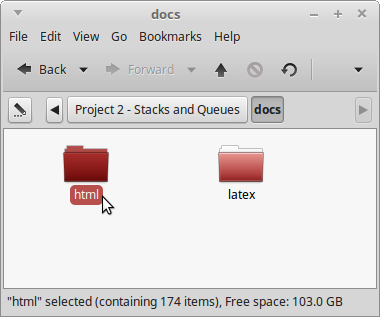
\includegraphics[width=6cm]{images/project2-docsfolder.png}
        \caption{Inside the docs folder}
    \end{figure}

    Then, open \textbf{index.html}.

    From the Index page, click on the \textbf{Classes} tab.
    This will open up a list of all the classes with documentation.

    \begin{figure}[h]
        \center
        \includegraphics[width=8cm]{images/classes.png}
        \caption{The Classes tab}
    \end{figure}

    Click on a class to view all its functions and the function specs.

    \newpage

    \begin{figure}[h]
        \center
        \includegraphics[width=8cm]{images/classlist.png}
        \caption{The list of classes in the documentation}
        
        ~\\
        \includegraphics[width=12cm]{images/doxygendocs.png}
        \caption{A function's documentation}

        ~\\
        \includegraphics[width=12cm]{images/doxygencode.png}
        \caption{Doxygen comments in the code}
    \end{figure}

    \newpage

% ----------------------------------------------------------------------
% ----------------------------------------------------------------------
% ----------------------------------------------------------------------
    \section{Testing}

    Before you start working with the actual program itself, you should
    develop your Binary Search Tree from within a project that uses
    unit tests.
    If you're using Code::Blocks, a CBP file is available in the
    \textbf{CodeBlocks Project - Tester} folder.

    ~\\
    If you're making your own project, the files you need to do testing are:

    \begin{itemize}
        \item   test\_main.cpp
        \item   BinarySearchTree.hpp
        \item   Tester.hpp
        \item   cuTEST/
        \begin{itemize}
            \item   TesterBase.hpp
            \item   TesterBase.cpp
            \item   StringUtil.hpp
        \end{itemize}
    \end{itemize}

    When you run the test, it will generate an output file called
    \textbf{test\_result.html} At first, its output will look like this:

    \begin{figure}[h]
        \center
        \includegraphics[width=14cm]{images/unit-test-output.png}
        \caption{Most unit tests fail}
    \end{figure}

    \newpage

    At the bottom of the page is the summary of all tests run:
    
    \begin{figure}[h]
        \center
        \includegraphics[width=12cm]{images/test-summary-bad.png}
        \caption{Most unit tests fail}
    \end{figure}

    Once everything passes, it will look like this:
    
    \begin{figure}[h]
        \center
        \includegraphics[width=12cm]{images/test-summary-good.png}
        \caption{Successful status at end}
    \end{figure}

    If there's a risk of a \textbf{segfault} (due to something returning
    null when it shouldn't), the test set will also cancel, not running all the tests:

    \begin{figure}[h]
        \center
        \includegraphics[width=12cm]{images/segfault-risk.png}
        \caption{Segfault risk causes tests to exit early}
    \end{figure}
    
    Make sure your tests all pass before getting into the program portion!

% ----------------------------------------------------------------------
% ----------------------------------------------------------------------
% ----------------------------------------------------------------------
    \section{Program}

    The program loads a list of employees from a text file.

    \begin{lstlisting}[style=textfile]
hamadi muruaga
	mission-critical-outside-the-box
	hotel-management-salesperson
	happy-alligator-754@sonnet.info

aboudou herppich
	synergistic-scaffolding
	legal-trainee
	faint-king-penguin-1574@telekinetic.com

kittie chamica
	synergistic-bandwidth
	metal-fabrication-director
	playful-centipede-1400@spiderweb.co.uk
    \end{lstlisting}

    The employees
    are stored in the \textbf{EmployeeManager} in three separate trees
    so that we can see how the indexing works for different types of keys.
    It also stores the employees in an unsorted \textbf{vector}.

    When you do a search for a specific employee, it the program will tell
    you how long it took to find them in the binary tree vs. how long
    it takes in the vector. For example:

    \begin{verbatim}
 LINEAR SEARCH TIME: 2.9768e-05 (microseconds) ... 3.1186e-05 (ticks)
 TREE SEARCH TIME:   2.912e-06 (microseconds) ... 3.373e-06 (ticks)
    \end{verbatim}

    \subsection{Example output}

    \paragraph{Program startup:} ~\\
    
    \begin{lstlisting}[style=output]
10000 employees loaded
id index generated, size 10000
name index generated, size 10000
email index generated, size 10000


1. Search by ID
2. Search by name
3. Search by email
4. Quit

>>
    \end{lstlisting}

    \paragraph{Searching by ID:} ~\\

    \begin{lstlisting}[style=output]
SEARCH BY ID
id: 30

EMPLOYEE FOUND:
EMPLOYEE ID: 30
	 FIRST NAME: nissrine
	 LAST NAME:  millet
	 JOB TITLE:  culinary-engineer
	 COMPANY:    immersive-deep-dive
	 EMAIL:      stark-x-ray-tetra-2799@cobweb.edu

	 LINEAR SEARCH TIME: 3.023e-06 (microseconds) ... 4.37e-06 (ticks)
	 TREE SEARCH TIME:   0.000152533 (microseconds) ... 0.000152954 (ticks)

    \end{lstlisting}
    
    \paragraph{Searching by name:} ~\\

    \begin{lstlisting}[style=output]
SEARCH BY NAME
lastname-firstname: nunn-mi

EMPLOYEE FOUND:
EMPLOYEE ID: 4
	 FIRST NAME: mi
	 LAST NAME:  nunn
	 JOB TITLE:  recording-arts-analyst
	 COMPANY:    empowering-outreach
	 EMAIL:      helpless-french-bulldog-1820@cobweb.info

	 LINEAR SEARCH TIME: 2.9768e-05 (microseconds) ... 3.1186e-05 (ticks)
	 TREE SEARCH TIME:   2.912e-06 (microseconds) ... 3.373e-06 (ticks)
    \end{lstlisting}
    
    \paragraph{Searching by email:} ~\\

    \begin{lstlisting}[style=output]
SEARCH BY EMAIL
email: playful-centipede-1400@spiderweb.co.uk

EMPLOYEE FOUND:
EMPLOYEE ID: 2
	 FIRST NAME: kittie
	 LAST NAME:  chamica
	 JOB TITLE:  metal-fabrication-director
	 COMPANY:    synergistic-bandwidth
	 EMAIL:      playful-centipede-1400@spiderweb.co.uk

	 LINEAR SEARCH TIME: 3.906e-06 (microseconds) ... 4.905e-06 (ticks)
	 TREE SEARCH TIME:   2.7e-06 (microseconds) ... 3.101e-06 (ticks)
    \end{lstlisting}


    \newpage

% ----------------------------------------------------------------------
% ----------------------------------------------------------------------
% ----------------------------------------------------------------------
    \section{Class declarations}

    \paragraph{Employee} ~\\

    \begin{lstlisting}[style=code]
struct Employee
{
    Employee();
    Employee( int newId, string newFirstName,
                string newLastName, string newCompany,
                string newJobTitle, string newEmail );
    void Display();

    int     id;
    string  firstName;
    string  lastName;
    string  company;
    string  jobTitle;
    string  email;
};
    \end{lstlisting}

    \paragraph{EmployeeManager} ~\\

    \begin{lstlisting}[style=code]
class EmployeeManager
{
public:
    EmployeeManager();

    void SearchById();
    void SearchByName();
    void SearchByEmail();

    void MainMenu();

private:
    void LoadEmployees();

    Employee* SearchById_Tree( int index );
    Employee* SearchByName_Tree( string name );
    Employee* SearchByEmail_Tree( string email );

    Employee* SearchById_Linear( int index );
    Employee* SearchByName_Linear( string name );
    Employee* SearchByEmail_Linear( string email );

    void GenerateIdIndex();
    void GenerateNameIndex();
    void GenerateEmailIndex();

    int GetIntInput( int min, int max );

private:
    vector<Employee> m_employeeList;

    BinarySearchTree<int, Employee*> m_idIndex;
    BinarySearchTree<string, Employee*> m_nameIndex;
    BinarySearchTree<string, Employee*> m_emailIndex;
};
    \end{lstlisting}

\newpage

    \paragraph{Node} ~\\

    \begin{lstlisting}[style=code]
        template <typename TK, typename TD>
        class Node
        {
        public:
            Node();
            ~Node();
            Node<TK, TD>* ptrLeft;
            Node<TK, TD>* ptrRight;
            TD data;
            TK key;
        };
    \end{lstlisting}

    \paragraph{BinarySearchTree} ~\\

    \begin{lstlisting}[style=code]
template <typename TK, typename TD>
//! A template binary search tree class
class BinarySearchTree
{
public:
    BinarySearchTree();
    ~BinarySearchTree();
    
    void Insert( const TK& newKey, const TD& newData );
    void Delete( const TK& key );
    bool Contains( const TK& key );
    string GetInOrder();
    string GetPreOrder();
    string GetPostOrder();
    TK* GetMax();
    int GetCount();
    int GetHeight();
    TD* GetData( const TK& key );

private:
    Node<TK, TD>* FindNode( const TK& key );
    Node<TK, TD>* FindParentOfNode( const TK& key );
    void RecursiveInsert( const TK& newKey,
        const TD& newData, Node<TK, TD>* ptrCurrent );
    void GetInOrder( Node<TK, TD>* ptrCurrent,
        stringstream& stream );
    void GetPreOrder( Node<TK, TD>* ptrCurrent,
        stringstream& stream );
    void GetPostOrder( Node<TK, TD>* ptrCurrent,
        stringstream& stream );
    TK* GetMax( Node<TK, TD>* ptrCurrent );
    int GetHeight( Node<TK, TD>* ptrCurrent );

private:
    Node<TK, TD>* m_ptrRoot;
    int m_nodeCount;

friend class Tester;
};
    \end{lstlisting}
    
% ----------------------------------------------------------------------
% ----------------------------------------------------------------------
% ----------------------------------------------------------------------
    \chapter*{Grading Breakdown}

    \textbf{Features}

    \begin{center}
        \includegraphics[height=14.5cm]{images/points-project3.png}
    \end{center}


\end{document}









